\documentclass[10pt,a4paper]{article}



% Basic packages only
\usepackage[top=0.2in, bottom=0.2in, left=0.5in, right=0.5in]{geometry}
\usepackage{enumitem}
\usepackage{titlesec}
\usepackage{graphicx}
\usepackage{multicol}
\usepackage{tikz}
\usepackage{tabularx}
\usepackage{array}
\usepackage{fontawesome5}
\usepackage{xcolor}
\usepackage{pagecolor}
\usepackage{fontspec}
\usepackage{microtype}
\usepackage{amsmath}



% Custom colors
\definecolor{bgcolor_color}{HTML}{423b28}
\definecolor{name_color}{HTML}{b9ad8c}
\definecolor{surname_color}{HTML}{877952}
\definecolor{title_color}{HTML}{b9ad8c}
\definecolor{blocktitle1_color}{HTML}{93d07c}
\definecolor{blocktitle2_color}{HTML}{669793}
\definecolor{blocktext1_color}{HTML}{B6E1E7}
\definecolor{blocktext2_color}{HTML}{3a7688}
\definecolor{linkcolor}{HTML}{43bbba}
\definecolor{skilltitle_color}{HTML}{93d07b}

\usepackage[colorlinks=true, linkcolor=linkcolor, urlcolor=linkcolor]{hyperref}
\newfontfamily\cambria{cambriab.ttf}[Path=fonts/]
\setmainfont{calibri.ttf}[Path=fonts/]

\titleformat{\section}
  {\normalfont\Large\bfseries\centering} % font size, bold, centered
  {} % no section number
  {0pt} % no extra spacing between label and title
  {} % what to insert before the title

\pagecolor{bgcolor_color} % sets full background
\color{blocktext1_color}

\newcommand{\sectionline}[1]{%
  \vspace{0.5em}
  \begin{center}
    \textcolor{title_color}{\rule[0.5ex]{0.25\linewidth}{0.5pt}}
    ~{\LARGE \bfseries \textcolor{title_color}{\cambria #1}}~
    \textcolor{title_color}{\rule[0.5ex]{0.25\linewidth}{0.5pt}}
  \end{center}
  \vspace{0.05em}
}


\newcommand{\circles}[2]{% #1 = filled, #2 = total
  \foreach \i in {1,...,#2} {
    \ifnum\i>#1
      \tikz\draw[gray,fill=none] (0,0) circle (1.2pt);
    \else
      \tikz\draw[black,fill=black] (0,0) circle (1.2pt);
    \fi
  }
}



\titlespacing*{\section}{0pt}{0.8em}{0.4em}
\setlist[itemize]{topsep=0pt, partopsep=0pt, itemsep=2pt, parsep=0pt}


\begin{document}

% Header
\vspace{-3em}
\noindent
\makebox[\textwidth][t]{%

% Column 1: Image
\begin{minipage}[c]{0.3\textwidth}
  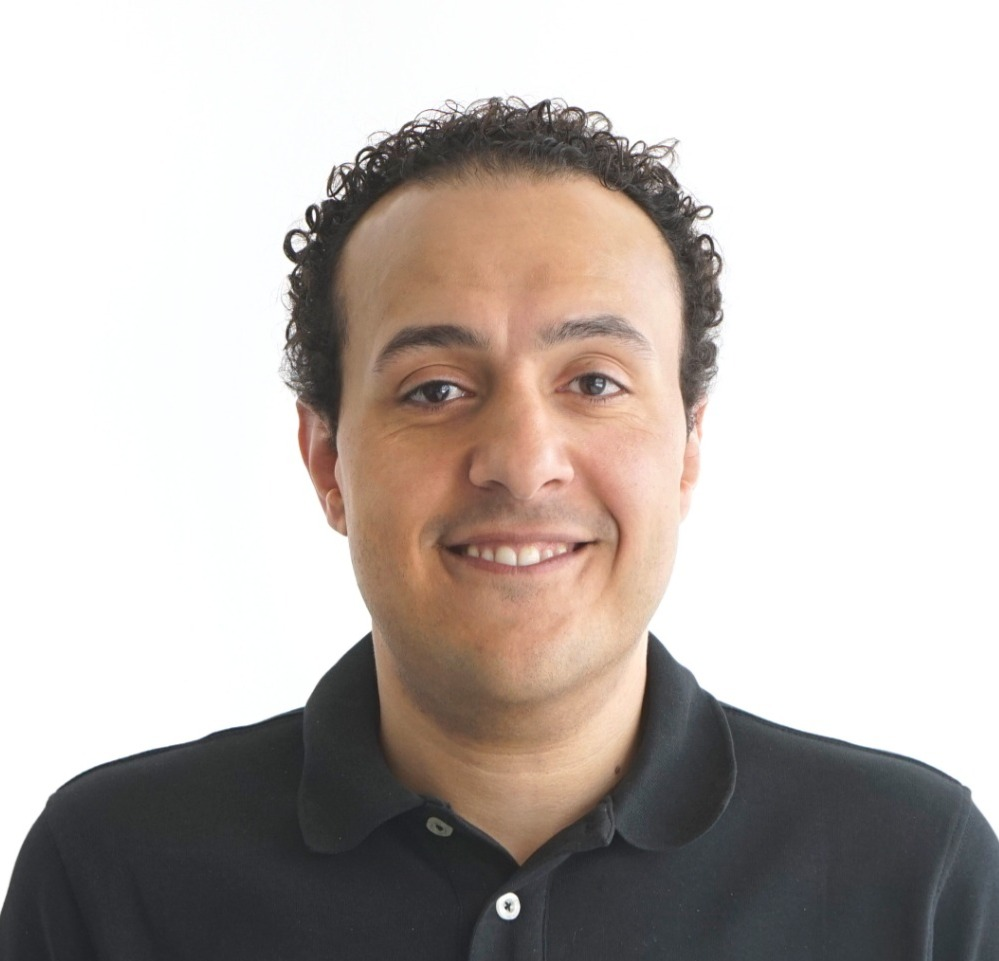
\includegraphics[width=0.8\linewidth]{images/my_image.jpg}
\end{minipage}%
\hspace{1em}

% Column 2: Name Block (baseline centered)
\begin{minipage}[c]{0.35\textwidth}
  {\fontsize{30pt}{32pt}\selectfont \textbf{\textcolor{name_color}{Amr}}}\\\\[-0.4em]
  \hspace{2.5em}{\fontsize{20pt}{22pt}\selectfont \textcolor{surname_color}{Aboughazala}}\\[0.8em]
\end{minipage}%
\hfill

% Column 3: Contact Info (forced to align at top)
\begin{minipage}[t]{0.35\textwidth}
  \begin{flushright}
    \textcolor{name_color}{\faEnvelope }\textcolor{linkcolor}{~\href{mailto:amr.abughazala@gmail.com}{amr.abughazala@gmail.com}}\\
    \textcolor{name_color}{\faPhone~+49 174 5969 482} \\
    \textcolor{name_color}{\faHome~Wieland Straße, Ulm, 89073} \\[1.5em]
    
    \textcolor{linkcolor}{\href{https://www.linkedin.com/in/amr-a-063776157/}{LinkedIn}} \quad
    \textcolor{linkcolor}{\href{https://www.xing.com/profile/Amr_Aboughazala/cv}{Xing}} \quad
    \textcolor{linkcolor}{\href{https://amr-aboughazala.super.site/}{Portfolio Site}}
  \end{flushright}
\end{minipage}%
}


% Objective
\sectionline{Objective}
\textcolor{blocktext1_color}{Bringing deep experience in R\&D and algorithm development, I aim to contribute to impactful work in signal processing, machine learning, perception, and computer vision within a research-focused environment.}

                      %% ---------------- R&D ---------------- %%
\sectionline{Key R\&D Contributions}
                             % ------ Scantinel Head ------ %

\begin{tabular}{@{}m{0.5cm}@{\hspace{0.5em}}m{2.2cm}@{\hspace{0.5em}}m{15cm}@{}}
  \raisebox{1.3em}{
\includegraphics[width=0.9cm]{images/scantinel_logo.png}} & 
  \raisebox{1.8em}{\begin{minipage}[t]{\linewidth}
  \centering
    \textcolor{blocktitle1_color}{Sep. 21}\\
    \textcolor{blocktitle1_color}{Present}
  \end{minipage} 
  } &
  \raisebox{0.5em}{\begin{minipage}[t]{\linewidth}
    \raggedright
    {\fontsize{11pt}{9pt}\selectfont\textbf{\textcolor{blocktitle1_color}{\text{Senior Algorithm and Data Processing Developer,}}}}
    {\fontsize{9pt}{9pt}\selectfont\textcolor{blocktitle2_color}{Scantinel Photonics GmbH, Ulm Germany}}
  \end{minipage}}
\end{tabular}

                         % ------ Scantinel Block ------ %
\vspace{0.3em}
\begin{itemize}[leftmargin=*]
  \item Led development and testing of the novel algorithm \href{https://amr-aboughazala.super.site/doppler-ambiguity-solution}{“VQRV”} for Doppler ambiguity in FMCW LiDAR systems.
  \item Proposed and implemented an internal perception pipeline (filtering, segmentation, object detection, tracking).\\ {\fontsize{10pt}{10pt}\selectfont\textcolor{blocktext2_color}{Sources: Ransac, knn, kd-tree, JPDA Tracking.}}. 
  \item Designed the Dense Cluster Filter “DCL” and the Multilevel Neighboring Filter “MLN”, improving performance from 450 ms to \href{https://amr-aboughazala.super.site/real-time-filtering}{“30 ms”} per frame.
  \item Created a \href{https://amr-aboughazala.super.site/data-analysis}{new confusion matrix} and evaluation scheme to evaluate raw time-domain and frequency-domain signal analysis.
\end{itemize}


                                  % ------ Navimatix Head ------ %
\vspace{1em}
\begin{tabular}{@{}m{0.5cm}@{\hspace{0.5em}}m{2.2cm}@{\hspace{0.5em}}m{15cm}@{}}
  \raisebox{1.3em}{
\includegraphics[width=0.9cm]{images/navi2_logo.png}} & 
  \raisebox{1.8em}{\begin{minipage}[t]{\linewidth}
  \centering
    \textcolor{blocktitle1_color}{Jan. 19}\\
    \textcolor{blocktitle1_color}{Jul. 21}
  \end{minipage} 
  } &
  \raisebox{0.5em}{\begin{minipage}[t]{\linewidth}
    \raggedright
    {\fontsize{11pt}{9pt}\selectfont\textbf{\textcolor{blocktitle1_color}{\text{Automated Image Analysis for Segmenting Bacteria,}}}}
    {\fontsize{9pt}{9pt}\selectfont\textcolor{blocktitle2_color}{Navimatix GmbH, Jena Germany}}
  \end{minipage}}
\end{tabular}


                                 % ------ Navimatix Block ------ %
\vspace{0.3em}
\begin{itemize}[leftmargin=*]
  \item A full pipeline image processing algorithms for bacteria counting on Fluorescence Images.\\ {\fontsize{10pt}{10pt}\selectfont\textcolor{blocktext2_color}{\fontsize{10pt}{10pt}\selectfont\textcolor{blocktext2_color}{Sources: Median Filter, ISODATA Segmentation, Opening Filter, 2D \& 3D counting}}}.
\end{itemize}

                             % ------ OBDient Head ------ %
                             
\vspace{1em}
\begin{tabular}{@{}m{0.5cm}@{\hspace{0.5em}}m{2.2cm}@{\hspace{0.5em}}m{15cm}@{}}
  \raisebox{1.3em}{
\includegraphics[width=0.9cm]{images/ilmenau1_logo.png}} & 
  \raisebox{1.8em}{\begin{minipage}[t]{\linewidth}
  \centering
    \textcolor{blocktitle1_color}{Jul. 18}\\
    \textcolor{blocktitle1_color}{Nov. 18}
  \end{minipage} 
  } &
  \raisebox{0.5em}{\begin{minipage}[t]{\linewidth}
    \raggedright
    {\fontsize{11pt}{9pt}\selectfont\textbf{\textcolor{blocktitle1_color}{\text{Kalman Filter on Satellite Reception,}}}}
    {\fontsize{9pt}{9pt}\selectfont\textcolor{blocktitle2_color}{Start Up OBDient, TU Ilmenau}}
  \end{minipage}}
\end{tabular}                             

                               % ------ OBDient Block ------ %
\vspace{0.3em}
\begin{itemize}[leftmargin=*]
  \item Implemented Kalman Filter GPS reception using a motion model of vehicles and pedestrians.
\end{itemize}                               

                             % ------ Master Thesis Head ------ %

\vspace{1em}
\begin{tabular}{@{}m{0.5cm}@{\hspace{0.5em}}m{2.2cm}@{\hspace{0.5em}}m{15cm}@{}}
\raisebox{1.3em}{
\includegraphics[width=0.9cm]{images/ilmenau1_logo.png}} & 
  \raisebox{1.8em}{\begin{minipage}[t]{\linewidth}
  \centering
    \textcolor{blocktitle1_color}{Mar. 17}\\
    \textcolor{blocktitle1_color}{Feb. 18}
  \end{minipage} 
  } &
  \raisebox{0.5em}{\begin{minipage}[t]{\linewidth}
    \raggedright
    {\fontsize{11pt}{9pt}\selectfont\textbf{\textcolor{blocktitle1_color}{\text{Positivity Decomposition Algorithms on EEG/MEG Data,}}}}
    {\fontsize{9pt}{9pt}\selectfont\textcolor{blocktitle2_color}{Master Thesis, MSCSP Group, TU Ilmenau}}
  \end{minipage}}
\end{tabular}                               

                                % ------ Master Thesis Block ------ %

\vspace{0.3em}
\begin{itemize}[leftmargin=*]
  \item Implemented non-negativity constraints on tensor-based blind source separation algorithm 
  \\ {\fontsize{10pt}{10pt}\selectfont\textcolor{blocktext2_color}{Sources:}} {\fontsize{10pt}{10pt}\selectfont\textcolor{blocktext2_color}{\href{https://ieeexplore.ieee.org/document/8313193}{Publication}}, {\fontsize{10pt}{10pt}\selectfont\textcolor{blocktext2_color}{\href{https://amr-aboughazala.super.site/non-negative-semi-algebraic-cp-decomposition-via-simultaneous-matrix-diagonalization}{Thesis Publication (not completed)}}}}
\end{itemize}


                             % ------ Siemens Head ------ %
                             
\vspace{1em}
\begin{tabular}{@{}m{0.5cm}@{\hspace{0.5em}}m{2.2cm}@{\hspace{0.5em}}m{15cm}@{}}
  \raisebox{1.3em}{
\includegraphics[width=0.9cm]{images/siemens4_logo.jpg}} & 
  \raisebox{1.8em}{\begin{minipage}[t]{\linewidth}
  \centering
    \textcolor{blocktitle1_color}{Sep. 16}\\
    \textcolor{blocktitle1_color}{Feb. 17}
  \end{minipage} 
  } &
  \raisebox{0.5em}{\begin{minipage}[t]{\linewidth}
    \raggedright
    {\fontsize{11pt}{9pt}\selectfont\textbf{\textcolor{blocktitle1_color}{\text{Technical Applications for time sensitive data AVB and TSN,}}}}
    {\fontsize{9pt}{9pt}\selectfont\textcolor{blocktitle2_color}{Work Student, Siemens, Network R\&D, Munich Germany}}
  \end{minipage}}
\end{tabular}                                

                                 % ------ Siemens Block ------ %
\vspace{0.3em}
\begin{itemize}[leftmargin=*]
  \item Implemented a simulation of TSN Scheduler as well as converter from SDN controller using C++.\\ {\fontsize{10pt}{10pt}\selectfont\textcolor{blocktext2_color}{\fontsize{10pt}{10pt}\selectfont\textcolor{blocktext2_color}{Sources: C++, Omnet++, }}} {\fontsize{10pt}{10pt}\selectfont\textcolor{blocktext2_color}{\href{https://1.ieee802.org/tsn/}{Time Sensitive Network for Industry v.4}}}.       
\end{itemize}              
                            
                                 

                             % ------ Advanced Research Head ------ %
\vspace{1em}
\begin{tabular}{@{}m{0.5cm}@{\hspace{0.5em}}m{2.2cm}@{\hspace{0.5em}}m{15cm}@{}}
  \raisebox{1.3em}{
\includegraphics[width=0.9cm]{images/ilmenau1_logo.png}} & 
  \raisebox{1.8em}{\begin{minipage}[t]{\linewidth}
  \centering
    \textcolor{blocktitle1_color}{Sep. 16}\\
    \textcolor{blocktitle1_color}{Feb. 17}
  \end{minipage} 
  } &
  \raisebox{0.5em}{\begin{minipage}[t]{\linewidth}
    \raggedright
    {\fontsize{11pt}{9pt}\selectfont\textbf{\textcolor{blocktitle1_color}{\text{Decomposition of a Low Rank Tensor with Missing Entries,}}}}
    {\fontsize{9pt}{9pt}\selectfont\textcolor{blocktitle2_color}{Advanced Research Project, MSCSP Group, TU Ilmenau}}
  \end{minipage}}
\end{tabular}                                  

                                % ------ Advanced Research Block ------ %
\vspace{0.3em}
\begin{itemize}[leftmargin=*]
  \item Developed a missing imputation tensor algorithm to make it adaptive as per step size and rank estimation.\\ {\fontsize{10pt}{10pt}\selectfont\textcolor{blocktext2_color}{Sources:}}  {\fontsize{10pt}{10pt}\selectfont\textcolor{blocktext2_color}{\href{https://amr-aboughazala.super.site/decomposition-of-a-low-rank-tensor-with-missing-entries}{document}}}.       
\end{itemize}              

                             % ------ Basic Research Head ------ %

\vspace{1em}
\begin{tabular}{@{}m{0.5cm}@{\hspace{0.5em}}m{2.2cm}@{\hspace{0.5em}}m{15cm}@{}}
  \raisebox{1.3em}{
\includegraphics[width=0.9cm]{images/ilmenau1_logo.png}} & 
  \raisebox{1.8em}{\begin{minipage}[t]{\linewidth}
  \centering
    \textcolor{blocktitle1_color}{Mar. 15}\\
    \textcolor{blocktitle1_color}{Jul. 15}
  \end{minipage} 
  } &
  \raisebox{0.5em}{\begin{minipage}[t]{\linewidth}
    \raggedright
    {\fontsize{11pt}{9pt}\selectfont\textbf{\textcolor{blocktitle1_color}{\text{Dynamic Speed Limit Scheme Using VANET Communication,}}}}
    {\fontsize{9pt}{9pt}\selectfont\textcolor{blocktitle2_color}{Basic Research Project, TU Ilmenau}}
  \end{minipage}}
\end{tabular}                                
                             
                               % ------ Basic Research Block ------ %
                               
\vspace{0.3em}
\begin{itemize}[leftmargin=*]
  \item Developed a scenario using Wireless Sensor Networks and VANETs. 
  \\ {\fontsize{10pt}{10pt}\selectfont\textcolor{blocktext2_color}{Sources: C++, Omnet++}}.       
\end{itemize}                                 
                               


                      %% ---------------- Technical Skills ---------------- %%
\sectionline{Technical Skills}
\hspace*{-1.5em}  % try -1em or adjust as needed
\noindent\makebox[\textwidth][c]{%
\begin{minipage}[t]{0.2\textwidth}
  \begin{center}
  \textbf{Languages}\\[0.5em]
  Python\\
  C++\\
  Java\\
  C\#\\
  Matlab
  \end{center}
\end{minipage}%
\hspace{1em}
\begin{minipage}[t]{0.65\textwidth}
  \begin{center}
  \textbf{Libraries}
  \end{center}
  \begin{minipage}[t]{0.4\textwidth}
    \textbf{DATA:} numpy, pandas, scipy\\
    \textbf{PLOT:} matplotlib, plotly, pyqtgraph\\
    \textbf{ML:} pytorch, scikit-learn, spconv\\
    \textbf{CV:} opencv
  \end{minipage}%
  \hfill
  \begin{minipage}[t]{0.5\textwidth}
    \textbf{VC:} git, gitlab\\
    \textbf{GUI:} PyQt, JavaFX, WPF\\
    \textbf{OOP:} MVC, MVVM\\
    \textbf{LIDAR:} open3D, open3DML, pytorch3d
  \end{minipage}
\end{minipage}%
\hspace{1em}
\begin{minipage}[t]{0.22\textwidth}
  \begin{center}
  \textbf{Technical Fields}\\[0.5em]
  Signal Processing\\
  Optimization\textendash{}Mathematics\\
  Machine Learning\\
  Wireless Communication\\
  Audio \& Image Processing\\
  Communication Networks
  \end{center}
\end{minipage}%
}



% Industry Experience
\newpage
\sectionline{Industry Experience}
\textbf{Senior Algorithm and Data Processing Developer} ~ Scantinel Photonics GmbH, Ulm Germany\\
\textit{Sept. 2021 -- Present}
\begin{itemize}[leftmargin=*]
  \item Led the architecture of new system software, collaborating with embedded teams to align hardware/software interfaces. skills: Pattern design MVC/MVVM 
  \item  Developed and maintained real-time and offline visualization GUIs supporting continuous feature development and release cycles for internal users and customers over two years. skills: python, PyQt 
  \item Built an offline testing platform for prototyping and analyzing signal processing pipelines. 
  \item implementing testing development creating unit, integration and functional testing. skills: pytest 
\end{itemize}

\vspace{0.6em}
\textbf{Software Developer} ~ Navimatix GmbH, Jena Germany\\
\textit{Jan. 2019 -- Jul. 2021}
\begin{itemize}[leftmargin=*]
  \item Developed a GUI applying image processing algorithm on Microscopic Images to count bacteria.
  \item Implemented several user interface applications. 
  \item Skills: JavaFX, .Net Framework WPF and Delphi.
\end{itemize}

\vspace{0.6em}
\textbf{ Sensors Expert and Data Analyst} ~ Start Up OBDient, TU Ilmenau\\
\textit{Jul. 2018 -- Jul. 2018}
\begin{itemize}[leftmargin=*]
  \item  Implemented data sensor fusion using GPS and Accelerometer on Raspberry Pi. Tools: NMEA Data of a NEO-6M GPS, MPU6050 GyroSensor, Raspberry Pi 3 B+ 
\end{itemize}

\vspace{0.6em}
\textbf{Customer Technical Network Specialist} ~ Orange Business Services, Cairo Egypt\\
\textit{Jul. 2011 -- Aug. 2014}
\begin{itemize}[leftmargin=*]
  \item Diagnose WAN network fault-related cases both proactive and reactive being responsible of the faults to resolution.
  \item Shift Leader for a group of 5 to 10 daily, managing the workflow through the team. 
\end{itemize}

% Education
\sectionline{Education}
\textbf{M.Sc. in Communications and Signal Processing}\\
Technische Universität Ilmenau, Germany\\
\textit{Sep 2014 -- Feb 2018}\\
Major: Mobile Communications, Adaptive Arrays, DSP\\
Grade: 2.2/1.0

\vspace{0.6em}
\textbf{B.Sc. in Electronics and Communication}\\
Arab Academy for Science and Technology, Alexandria\\
\textit{Sep 2007 -- Feb 2010}\\
Grade: 1.3/1.0 — Top of class

% Courses
\sectionline{Certificates and Online Courses}
\begin{itemize}[leftmargin=*]
  \item 22 May 2019: \href{https://www.udemy.com/certificate/UC-XN2ILPOB/}{OOP in Java — Udemy}
  \item 24 Aug. 2020: \href{https://coursera.org/share/e32b80d8e0b32b48e4ad6fe40cea746e}{Machine Learning — Coursera}
  \item 14 May 2021: \href{https://coursera.org/share/15d74342746d2872a09dcc5a75ff460c}{Structuring ML Projects — Coursera}
  \item 30 Apr. 2021: \href{https://coursera.org/share/0ca157f56b99f56122ab247589555837}{Neural Networks and Deep Learning — Coursera}
  \item 04 Jun. 2021: \href{https://coursera.org/share/e0bd7b6ea301e1108dfe609c783f2706}{Convolutional Neural Networks — Coursera}
  \item 07 May 2021: \href{https://coursera.org/share/ef6671ff524b9d2e5c1e0e282d457f56}{Improving DNN Hyperparameter Tuning, Regularization and Optimization — Coursera}
  \item 24 Aug. 2021: \href{http://www.udacity.com/certificate/e/95ce8498-c21f-11eb-aa1a-5f098308d726}{Sensor Fusion — Udacity (Mercedes Benz)}
\end{itemize}


\vspace{2em}
\sectionline{Personal Skills}

\begin{center}
\begin{minipage}[t]{0.45\textwidth}
  \centering
  \textbf{Languages}\\[0.5em]
  Arabic: Native\\
  English: Fluent\\
  German: B1 TELC\\
    {\footnotesize
    Hören \quad \circles{2}{6}\\
    Lesen \quad \circles{2}{6}\\
    Schreiben \quad \circles{2}{6}\\
    Sprechen \quad \circles{2}{6}\\
    }

\end{minipage}%
\hfill
\begin{minipage}[t]{0.45\textwidth}
  \centering
  \textbf{Interests}\\[0.5em]
  Graphics Design\\
  Tennis\\
  Movies and TV Series\\
  Trying Different Restaurants
\end{minipage}
\end{center}


\end{document}